\abstracttitle{Exascale Systems}
\abstractauthor[Kenneth Moreland and Dirk Pleiter]{%
Kenneth Moreland (Sandia National Laboratories -- Albuquerque, kmorel@sandia.gov)\\
Dirk Pleiter (Jülich Supercomputing Centre, d.pleiter@fz-juelich.de)
}

\license

\wgpar{Contributors:} T. Peterka, K. Moreland, K. Isaacs, B. Muite, D. Pleiter, B. Raffin, U.  Rüde, R. Sisneros, G. H. Weber

\begin{refsection}

\wgpar{Background and Motivation}
%What is the problem [from the point of view of in situ]?
The exascale system represents many paradigm shifts that absolutely necessitate the shift to in situ analysis and visualization. Already well established by the visualization community, and backed up by many applications scientists~\cite{Gerber18}, is the need of in situ visualization as a response to the growing gap between compute rate and disk storage bandwidth.
We expect other relevant fundamental changes to HPC processing at the exascale. HPC workload is shifting from a traditional solver PDE workload to a mixture of multiple physics, analytics, visualization, learning, and other complex processing units. For in situ visualization to be viable in this complex software ecosystem, we must better understand exascale system requirements for in situ applications; we must map application needs to system and analysis features, and we must identify gaps in current HPC systems for a set of in situ workloads viable for the exascale.

\wgpar{Challenges.}
HPC design and its use are a shifting target. HPC design, both known and unknown, present both interesting challenges and opportunities.
It is generally observed that the throughput of floating-point operations is increasing at a much higher speed compared to I/O bandwidth, such that their ratio seems to increase exponentially (see Fig.~\ref{fig:44}, left panel). That is, I/O to an external storage system becomes ever more challenging. Newly presented to the community is the observation that maintaining a high aggregate memory bandwidth became challenging, too, resulting in a decline of the ratio of throughput of floating-point operations and memory bandwidth (see Fig.~\ref{fig:44}, right panel). This may be in part to a (possibly temporary) trend in using fewer nodes per computer (thus indirectly reducing the total number of memory buses). Regardless, it is worthwhile to closely monitor this trend as its behavior may drastically affect the consequential research of in situ visualization. For example, perhaps integrating visualization too tightly with simulation may divide an already constrained bandwidth. One option to mitigate the memory bandwidth challenge is to use new high-bandwidth memory technologies like HBM, which are currently, for example, used for high-end GPUs. For cost reasons this may, however, result in a degradation of the available memory capacity.

\begin{figure}[t]
	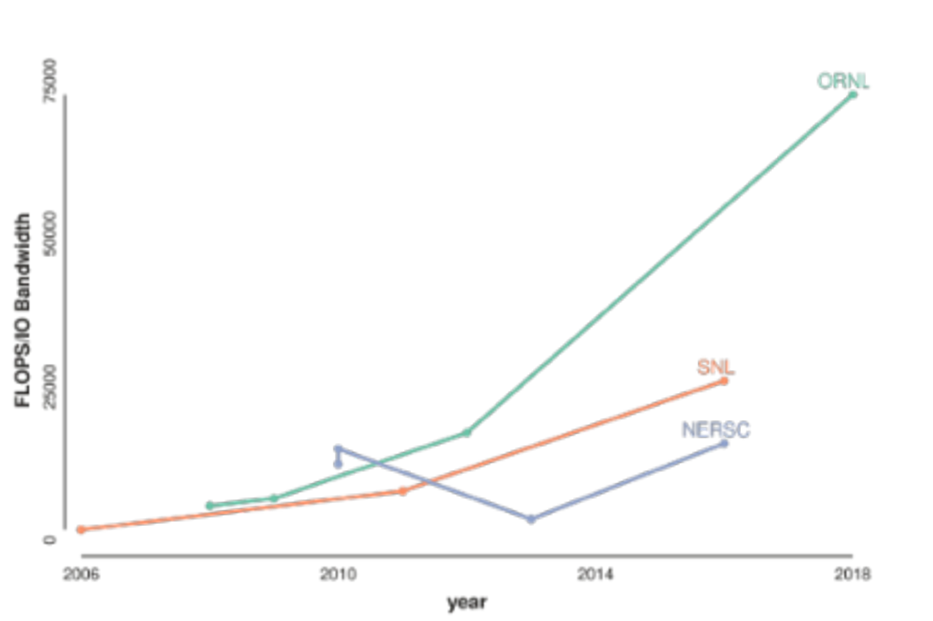
\includegraphics[width=.45\textwidth]{fig-44L} \space{5mm}	
	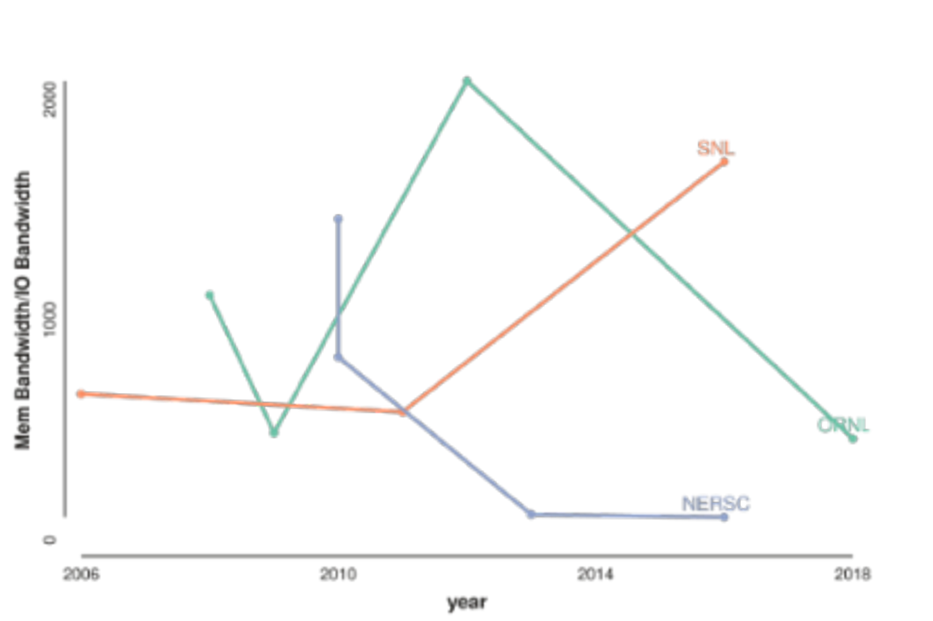
\includegraphics[width=.45\textwidth]{fig-44R}
	\caption{At left is a plot of the FLOPS to disk I/O bandwidth for the last three generations of computers at ORNL, NERSC and SNL/LANL respectively. At right is the ratio of the memory bandwidth to disk I/O bandwidth for the same computers.\label{fig:44}}
\end{figure}

A possible strategy for mitigating the capacity problem is the integration of persistent memory, which appears to be a common theme for exascale systems in a variety of forms. One such well documented application for persistent memory is the concept of burst buffers \cite{Bent12}, which provides storage areas typically based on non-volatile memory (NVRAM) like NAND Flash as a staging area for slower external storage. Such buffers may provide an opportunity to intercept simulation data at a lower cost than that of a disk-based storage system. Another opportunity includes the integration of NVRAM into the compute nodes, where it could either be attached to the processors as a storage device or as memory. Although the non-volatile aspect of NVRAM may be secondary to high density (and thus high storage capacity) and low storage power for the base applications \cite{Caulfield10}, the introduction of such memory may open up many opportunities such as the injection of in transit visualization capabilities while memory is staged.

As the scale of supercomputers increase, the feasibility of building dedicated visualization clusters decreases \cite{Childs07}. However the possibility of providing heterogeneous nodes in new supercomputers specialized for analysis and visualization processing still remains. Such dedicated nodes integrated into the rest of the supercomputer fabric enables much in situ processing, particularly of the in transit variety.
As the complexities of simulations advance and in situ visualization is incorporated into the workflow, understanding the performance behavior of visualization algorithms becomes more critical. Currently, the performance behavior of in situ systems is not well understood, and in fact the number of potential in situ approaches and implementations are too vast to effectively study. Although research in new in situ approaches should continue to remain a priority, we need to downselect the potential space of probable in situ possibilities to the most probable (and effectively implemented) solutions to really measure performance.
We also recognize that exascale and post-exascale machine definitions are not set. This gives the visualization community an opportunity to provide input to decision makers on what features should be provided by upcoming systems. Such recommendations can only be given if the performance of (the aforementioned downselected) in situ visualization capabilities are well understood.

\wgpar{Successes.}
There has been some introductory work on performance modeling of visualization algorithms, but much more remains to be done. Tools like Ascent~\cite{Larsen17} and SENSEI~\cite{Ayachit16} provide small sample applications that can be used for targeted studies of performance. For a formalized study, we first need an ontology of in situ techniques to guide the experiments performed. The In Situ Terminology Project~\cite{ISTP} provides a classification system that breaks down current in situ visualization techniques. See Section~\ref{sec:costModels} on cost models for more information.
We endeavor to make in situ visualization capabilities an integral part of the design of an overall exascale system. Generally, co-design is used to ensure that future generations of supercomputers are well-suited to the applications to be run on them. Although visualization needs have previously been poorly represented, the model of co-design with science applications is an established model we can apply to our needs. As in situ visualization becomes more critical for scientific computation, we expect to be in better position to be included in co-design efforts. Co-design has become an established methodology towards exascale computing (see, e.g., \cite{Barrett13}). In a co-design process, application and system software developers make their needs and requirements available to system architects. On this basis these will be able to identify the most efficient solutions and perform trade-off decisions. On the other hand, system architects and system technology experts should provide application and system software developers with expertise on both limitations of the underlying architecture and technologies as well as opportunities, which could be exploited. 
One example where co-design could be beneficial is the aforementioned NVRAM integration. Know-how on key performance characteristics, realisable memory capacities and possible access interfaces will empower developers of in situ visualisation software about design solutions, which could allow to efficiently exploit this NVRAM. Defining the needs of workflows involving in situ visualisation components will allow system architects to choose between different NVRAM solutions as well as APIs for accessing this memory.

\wgpar{Research Questions.} 
To be successful in a co-design for future computing platforms, it is important to express needs and desires at an appropriate level with metrics that are meaningful to vendors. For example, in the context of co-design it is a poor idea to express a requirement in the form of a need for a burst buffer because doing so is unnecessarily prescriptive to a particular technology when another technology may satisfy the needs as well or better. Instead, the focus should be on defining needs and requirements, e.g. in terms of needing N amount of memory capacity with M amount of bandwidth for a duration of T time. Research might also identify potentially new elements, such as containers, that expand the capabilities of in situ visualization and ease the integration of such components.
The current state of the art in visualization is quite poor at predicting the system needs of our own systems in isolation let alone understanding how they perform in a larger in situ workflow or when mapped to differentsystem components. 

Our first task in understanding visualization performance better is to come up with an ontology of classes of general in situ processing. The In Situ Terminology Project has already identified 6 separate (but interdependent) axes of in situ features with each axis containing many potential values, and for the most part the terminology does not detail the actual analysis and visualization algorithms to be run. This expansive space is likely too vast to densely measure, so a certain amount of downselecting is important to identify the classes of in situ visualization most likely to be employed in practice. That is not to say that research of possible in situ solutions should similarly be constrained, and such unconstrained research may in turn adjust the priorities considered for supercomputer co-design. However, when building cost models this downselection is important to make the problem tractable.

There are numerous expected features of exascale computing that will prove challenging. As ever, the next generations of supercomputers will feature more parallelism: potentially many thousands of nodes and an aggregate of billions of computing threads. In situ visualization exacerbates the challenge by requiring the visualization to run on more computing threads than strictly necessary. This is because even large visualizations are traditionally run at smaller scales than the simulation (rule of thumb dictates 5-10\% the size). Consequently, visualization run in situ either needs to take a leap in the scalability of the software or employ in situ techniques that separates visualization processing to smaller computing groups.

New memory structures, types, and hierarchies are also expected to provide numerous challenges and opportunities. As NVRAM continues to become more cost effective, their use in supercomputers will likely expand. Using NVRAM in SSD form for storage components like burst buffers remains a potential use case, but NVRAM may be considered in different ways as well. For example, their high data density and ability to retain data at low power make them attractive as a potential component of the addressable memory system, which could allow them to double as a communication mechanism between workflow components (such as simulation and visualization).

Also of note about the memory system is the observation that, although in situ research has primarily focused on the growing gap between throughput of floating-point operations and storage bandwidth, a similar trend can be seen between execution rate and the RAM memory bandwidth. As we use in situ visualization to move analysis closer to simulation, we may be exacerbating problems with limited memory bandwidth in favor of relieving storage bandwidth. It is an open question of how much, if at all, an in situ visualization affects the available memory bandwidth to other workflow functions and, if so, how the work may be divided across different memory busses.

\wgpar{Conclusion.}
Addressing these issues will enable better support of in situ visualization on exascale supercomputers and beyond. A better understanding of the behavior of our own visualization systems will allow us to both steer future HPC design to better enable and, conversely, adjust in situ visualization R\&D to better perform on available platforms. Ultimately, such research and co-design will lead to more effective application of in situ visualization.

\printbibliography
\end{refsection}

